%===================================== CHAP 4 =================================

\chapter{Data}
For our analyses we have gathered data on the  S\&P 100 companies. For each company we have collected price data, trading volumes, news article counts, Google Trends data, and Wikipedia pageviews.  
\\\\
We include all companies that were part of S\&P 100 as of October 1, 2018, except Dow DuPont, Booking Holdings and Walgreens Boots Alliance, as they lack Google Trends data. For concept trend, Dow Dupont does not exist in Google Trends, while Booking Holdings only has data from February 2018. Walgreens Boots Alliance had null values in the dataset for concept trend, which gives invalid values in our dataset. After removing companies with incomplete data we were left with 97 companies and 7275 observations. A complete list of the stock tickers we use in our analyses is given in Appendix \ref{app:company_terms}.


\section{News articles}\todo{si noe om hvor mye vi har lastet ned}
News articles are collected from the Thomson Reuters Eikon database where we are able to obtain news articles categorized by the companies they mention. Our dataset covers the time period between July 2017 and September 2018 for both information demand and supply variables. This is about the same time period as \cite{vlastakis} use for the information supply variable in their analyses. The Thomson Reuters Eikon database provides detailed news data and its website provides the following description of the news database:
\\
"Access content from over 400 real-time streaming news sources and financial newswires, over 6,000 near real-time and archived sources, and hundreds of Web sources so that you have the full spectrum of information you need to act first. All regions of the world are covered, including essential emerging markets." (\cite{descriptionThomsonReutersdatabase})
\\\\\todo{nevn antallet nyhetskilder brukt, average/max/min, totalt antall artikler in our database}
In Thomson Reuters we use Reuters instrument codes (RICs) instead of company names when collecting news articles. RICs allow us to  gather news articles that relates to subsidiaries of a company without doing multiple manual searches for each of them. To extract the news data we wrote a script accessing the Eikon API. It obtains all news articles from the NewsWire and NewsRoom databases, which are tagged as mentioning one of the S \& P 100 companies. For each company we make a weekly count of the number of articles who are tagged with the company RIC.
\\\\
\todo{skriv noe mer om scriptingen/applikasjonen, hva kan den gjoere?}
To normalize news data we transform weekly news count, $Nws$, into the Abnormal News Count with the following formula:
\begin{equation}
   \label{abnormal_news} 
   AbnNws_{t} = log(Nws_{t}) - log[Med(Nws_{t-8},...,Nws_{w-1})] 
\end{equation}
\\
where $log(Nws_{t})$ is the logarithm of the news count at week number $t$. $log[Med(Nws_{t-8},...,Nws_{t-1})]$ is the logarithm of the median $Nws$ for the previous 8 weeks in accordance with \cite{engelberg}. 
\\\\
$log$ is defined as the natural logarithm in all equations. 
\\\\
\section{Company financials}
Daily company financials are obtained from the Alpha Vantage API using ticker codes for each company. This includes open, close, high, low, adjusted close, and volume for each ticker. We use weeks starting and ending on Mondays when calculating financial variables. This is to make sure all variables have comparable time periods. As Google Trend uses weeks starting on Sunday and ending on Saturday, Monday is the first available trading day after the Google Trends week ends. 
\subsection*{Log return}
We use Equation \eqref{log_return} to calculate the weekly log return:
\begin{equation}
   \label{log_return} 
   R_t = log (C_{t+1}/C_{t}) 
\end{equation}
where $C_{t}$ is the adjusted Monday closing price and $R_{t}$ is the return for week $t$.
\\\\
\subsection*{Trading volume}
We use the following equation to calculate the daily Abnormal Trading Volume ($AbnVlm$) for a company: 
\begin{equation}
   \label{abnormal_volume} 
   AbnVlm_{t} = log(Vlm_{t}) - log[Med(Vlm_{t-8},...,Vlm_{t-1})] 
\end{equation}
   where $AbnVlm_t$ is the Abnormal Trading Volume at week $t$. $log(Vlm_{t})$ is the logarithm of the trading volume at week $t$. $log[Med(Vlm_{t-8},...,Vlm_{t-1})]$ is the logarithm of the median $Vlm$ for the previous 8 weeks.
\subsection*{Volatility}
We use the \cite{garman} volatility estimator adjusted for opening jumps as discussed in \cite{molnar_volatility}.
The following formula is used to calculate daily variance:
\begin{equation}
   \label{w_volatility} 
    \sigma^2_{d} = \frac{1}{2}(h_d-l_d)^2-(2log(2)-1)c_d^2+jadj_d^2
\end{equation}
with:
\begin{equation}
\begin{split}
c_{d} = log(close_{d})-log(open_{d}) \\
l_{d} = log(low_{d})-log(open_{d}) \\
h_{d} = log(high_{d})-log(open_{d}) \\
j_{d} = log(open_{d})-log(close_{d-1}) \\
r_{d} = log(close_{d})-log(close_{d-1}) \\
radj_{d} = log(aclose_{d})-log(aclose_{d-1}) \\
jadj_{d} = j_{d} \frac{radj_{d}}{r_{d}} \\
\end{split}
\end{equation}
Weekly variance is calculated as:
\begin{equation}
   \label{w_volatility} 
    \sigma^2_{t} = \sum_{d \in t} \sigma^2_{d} 
\end{equation}
Finally weekly volatility is calculated as:
\begin{equation}
   \label{w_volatility} 
    \sigma_t = \sqrt{\sigma^2_t}
\end{equation}
 where t is week number. $high_{d}$ and $low_{d}$ is the highest and lowest quoted price on the given day, and $open_{d}$, $close_{d}$, $aclose_{d}$ is the open, close and adjusted close price on the given day. 

\section{Search volume}\label{sec:search volume}\todo{legg inn bilder av ticker, search term og name -> beveger seg ulikt, ulikt antall klikk}
\todo{en som viser size difference}
\todo{en som viser ulike bevegelser}
Search volume data is collected from Google Trends which provides data about Google search volume for keywords or concepts. The search volume data is downloaded directly from the Google Trends page. The index is reported as a value between 0 and 100 for the given time period. The Search Volume Index (hereafter called SVI) values are normalized based on the chosen time interval during download, so the highest value equals 100. The SVI values are not meaningful in themselves, as they can be be manipulated to an arbitrary number by changing the time interval. Therefore, it is necessary to standardize the values. Standardization also makes the index more comparable across companies. We standardize by taking the logarithm of the SVI minus its median in the first 8 weeks. 
\\\\
We collect 3 different Google Trends SVI's per company:
\\\\
\textit{Ticker trend}
\\
Using each companies stock ticker as a keyword
\\\\
\textit{Search term trend}
\\
We follow the method described in  \cite{vlastakis}. We started by inserting the full company name and all the variations known to us to Google Insights for Search and chose the keyword with the largest search volume.
\\\\
\textit{Concept trend}
\\
\todo{legge inn forklaring på hvordan vi fant concept trend, deler av lenke: bilde av url og hvilken del som klippes ut. setter inn i dekoderlenke og får ut concept trend id.}Concept trend is a recently introduced search function in Google Trends. We find the concept id for each company by searching on the company name in Google Trends and choosing the company result instead of the search term. In some cases, where a holding company consist almost exclusively of a daughter company the daughter company is used instead.
\\\\
When searching for keywords, only searches matching the specific spelling and language is returned. This can be a problem if the company name is hard to spell, or is used in different ways ”Concepts” tries to overcome this problem by grouping all keywords and translations relevant to a specific ”concept” together. This gives a far broader and potentially more accurate picture of the interest in the ”concept”.
\\\\
For a complete list of company identifiers see Appendix \ref{app:company_terms}
\\\\
We use Equation \eqref{log_asvi} to calculate the Abnormal Search Volume Index ($AbnSVI$) at week $t$:
\begin{equation}
   \label{log_asvi} 
   AbnSVI_{t} = log(SVI_{t}) - log[Med(SVI_{t-8},...,SVI_{t-1})] 
\end{equation}
where $log(SVI_{t})$ is the logarithm of the Search Volume Index at week $t$. $log[Med(SVI_{t-8},...,SVI_{t-1})]$ is the logarithm of the median $SVI$ for the previous 8 weeks.
\\\\
It is interesting to include three different trends data from Google for each company, as the companies show different movements for company trend, search term trend and ticker trend. An example of this can be seen in figure \ref{fig:bmyStatisticsGoogleTrends} for Bristol-Myers Squibb. In figure \ref{fig:bmyStatisticsGoogleTrends}, the movements in company trends is quite different from the movements in ticker trend. Further, the search volume for company trend, ticker trend and search term trend is different for a company as well. In figure \ref{fig:xomStatisticsGoogleTrends} we see that search volume for company trend is more than twice as large as it is for the search term trend. Because movements and search volume fluctuate across ticker trend, search term trend and company trend for a specific company, it is likely that they contain different information.   
\begin{figure}[h!]
  \centering
    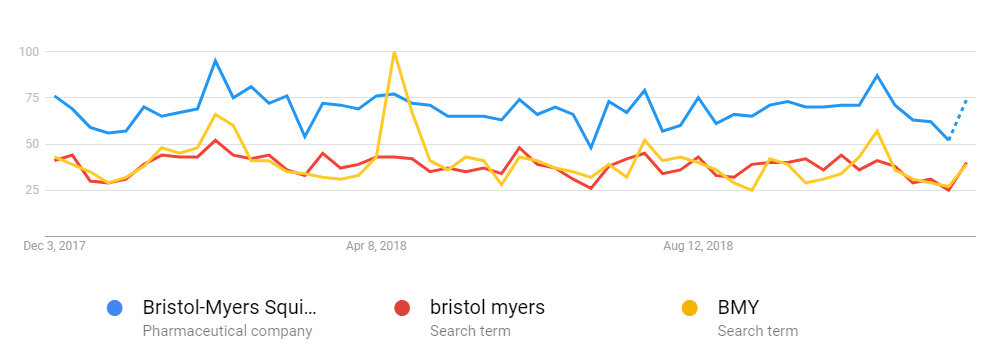
\includegraphics[width=1\textwidth]{fig/bmyStatisticsGoogleTrendsAddedExplanation.png}
 \caption{Google Search Volume for company trend, ticker trend and search term trend for Bristol-Myers Squibb.}
\label{fig:bmyStatisticsGoogleTrends}
\end{figure}
\begin{figure}[h!]
  \centering
    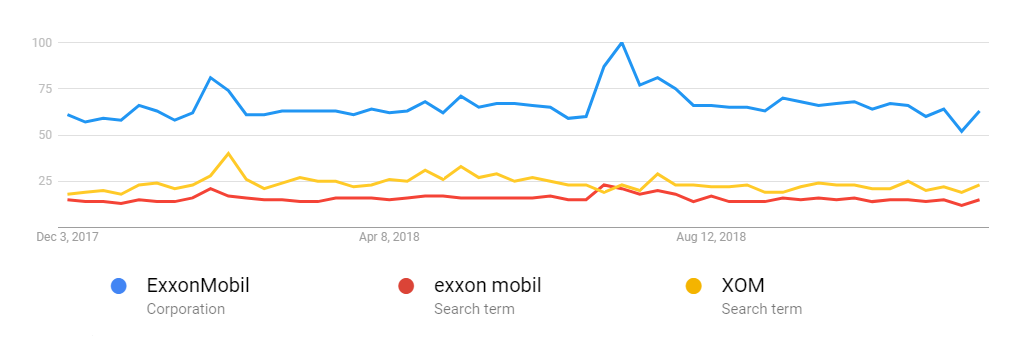
\includegraphics[width=1\textwidth]{fig/xomStatisticsGoogleTrendsAddedExplanation.png}
 \caption{Google Search Volume for company trend, search term trend and ticker trend for Exxon Mobil.}
\label{fig:xomStatisticsGoogleTrends}
\end{figure}

\section{Wikipedia views}

Wikipedia views are collected from Wikipedia Pageviews Analysis which is is a tool to extract pageview volume for individual Wikipedia pages. Pageviews Analysis gives us the absolute view counts on the pages for each of the S\&P 100 companies on a daily, weekly and yearly basis. To get company specific data we map company names to the Wikipedia pages describing them.
\\\\
We use Equation \eqref{log_asvi} to calculate the Abnormal Pageviews Volume ($AbnWiki$) at week $t$, which is basically the same equation as Equation \eqref{abnormal_volume}:
\begin{equation}
   \label{abnormal_pageviews_volume} 
   AbnWiki_{t} = log(Wiki_{t}) - log[Med(Wiki_{t-8},...,Wiki_{t-1})] 
\end{equation}
   where $log(Wiki_{t})$ is the logarithm of the Pageviews Volume at week $t$, and $log[Med(Wiki_{t-8},...,Wiki_{t-1})]$is the logarithm of the median $Wiki$ for the previous 8 weeks.
\todo{Figure with data for interest in company from wiki, trends and news articles (add some text, ulikhet gjør det interessant å ta med alle variablene i analysen, da de gir oss forskjellig bilde av information demand, inneholder samme info med ulike støykilder)}
\section{Monthly variables}
% TODO write about normalisation of stdev and calculation of monthly variables
 We also calculate the monthly average for all variables by taking the average over the last 4 weeks. 
\begin{equation}
   \label{monthly_var} 
   variable^{m}_t = avg(variable^{w}_{t},...,variable^{w}_{t-3}) 
\end{equation}
where $m$ and $w$ indicate monthly and weekly variables. The reason to include monthly variables is to allow for longer term dependencies in variables. Instead of including several lagged variables we are using monthly variables to keep the model parsimonious.
\\\\
Finally, all variables, including monthly averages, are normalized to have a standard deviation of 1 across the pooled data. Normalization makes the coefficients easier to compare across variables and regression models.
\todo{avsnitt om innsamlingen av data med scriptingen (API, Pandas}
\todo{Oppdater tabell}
\section{Descriptive statistics}
\begin{table}[!htbp] \centering 
  \caption{Descriptive statistics} 
  \label{tab:desc_stat} 
\begin{tabular}{@{\extracolsep{5pt}}lcccccc} 
\\[-1.8ex]\hline 
\hline \\[-1.8ex] 
Statistic & \multicolumn{1}{c}{Mean} & \multicolumn{1}{c}{St. Dev.} & \multicolumn{1}{c}{Min} & \multicolumn{1}{c}{Pctl(25)} & \multicolumn{1}{c}{Pctl(75)} & \multicolumn{1}{c}{Max} \\ 
\hline \\[-1.8ex] 
log\_return & 0.002 & 0.031 & $-$0.209 & $-$0.013 & 0.020 & 0.224 \\ 
w\_vol & 0.010 & 0.004 & 0.003 & 0.007 & 0.012 & 0.049 \\ 
logmedian\_VOLUME & 0.017 & 0.341 & $-$1.307 & $-$0.199 & 0.207 & 1.875 \\ 
logmedian\_news\_count & 0.026 & 0.657 & $-$4.635 & $-$0.305 & 0.335 & 5.513 \\ 
logmedian\_wiki & 0.025 & 0.195 & $-$0.953 & $-$0.061 & 0.075 & 2.629 \\ 
logmedian\_concept\_trend & 0.004 & 0.150 & $-$0.869 & $-$0.053 & 0.047 & 2.813 \\ 
logmedian\_search\_term\_trend & 0.002 & 0.146 & $-$1.030 & $-$0.056 & 0.054 & 1.966 \\ 
logmedian\_ticker\_trend & 0.009 & 0.197 & $-$3.738 & $-$0.056 & 0.054 & 1.833 \\ 
\hline \\[-1.8ex] 
\end{tabular} 
\end{table} 

\clearpage

\subsection*{Stationarity}
% Stationarity test are run from the stationarity_test Jupyter file

The log-median transformation should correct for non-stationary effects in the original data. 
Subtracting previous values removes any linear trend, and taking the logarithm should minimize other non-linear relations. 
\\\\
To test for stationarity in the transformed variables we run the argumented Dickey-Fuller (ADF) test for each variable and each company separately. The test indicates stationarity for all variables after normalization. 
\\\\
Volatility is not tested under ADF as it is known to be autoregressive, it will therefore almost certainly fail an ADF test. 










